\section{Results}
\label{sec:results}

\subsection{Corrupted evidence}
\label{sec:res-corrupt}

Figure~\ref{fig:corruption} shows how each quantity changes as more of the numbers in the retrieved evidence are replaced.
Accuracy falls steeply: averaged over runs, from \accZeroFin{} to \accFullFin{} on FinQA and from \accZeroTat{} to \accFullTat{} on TAT-QA.
Numeric-overlap support computed against the evidence the model was shown barely changes (FinQA \ovZeroFin{} to \ovFullFin{}, TAT-QA \ovZeroTat{} to \ovFullTat{}), as does entailment support and the hallucination flag.
The reason is mechanical: the model copies the corrupted figures it was shown into its reasoning, and those figures are in the evidence.
Support computed against the \emph{clean} evidence falls from \vscZeroFin{} to \vscFullFin{} on FinQA and from \vscZeroTat{} to \vscFullTat{} on TAT-QA, because the copied figures are not in the clean evidence.

\begin{figure}[t]
\centering
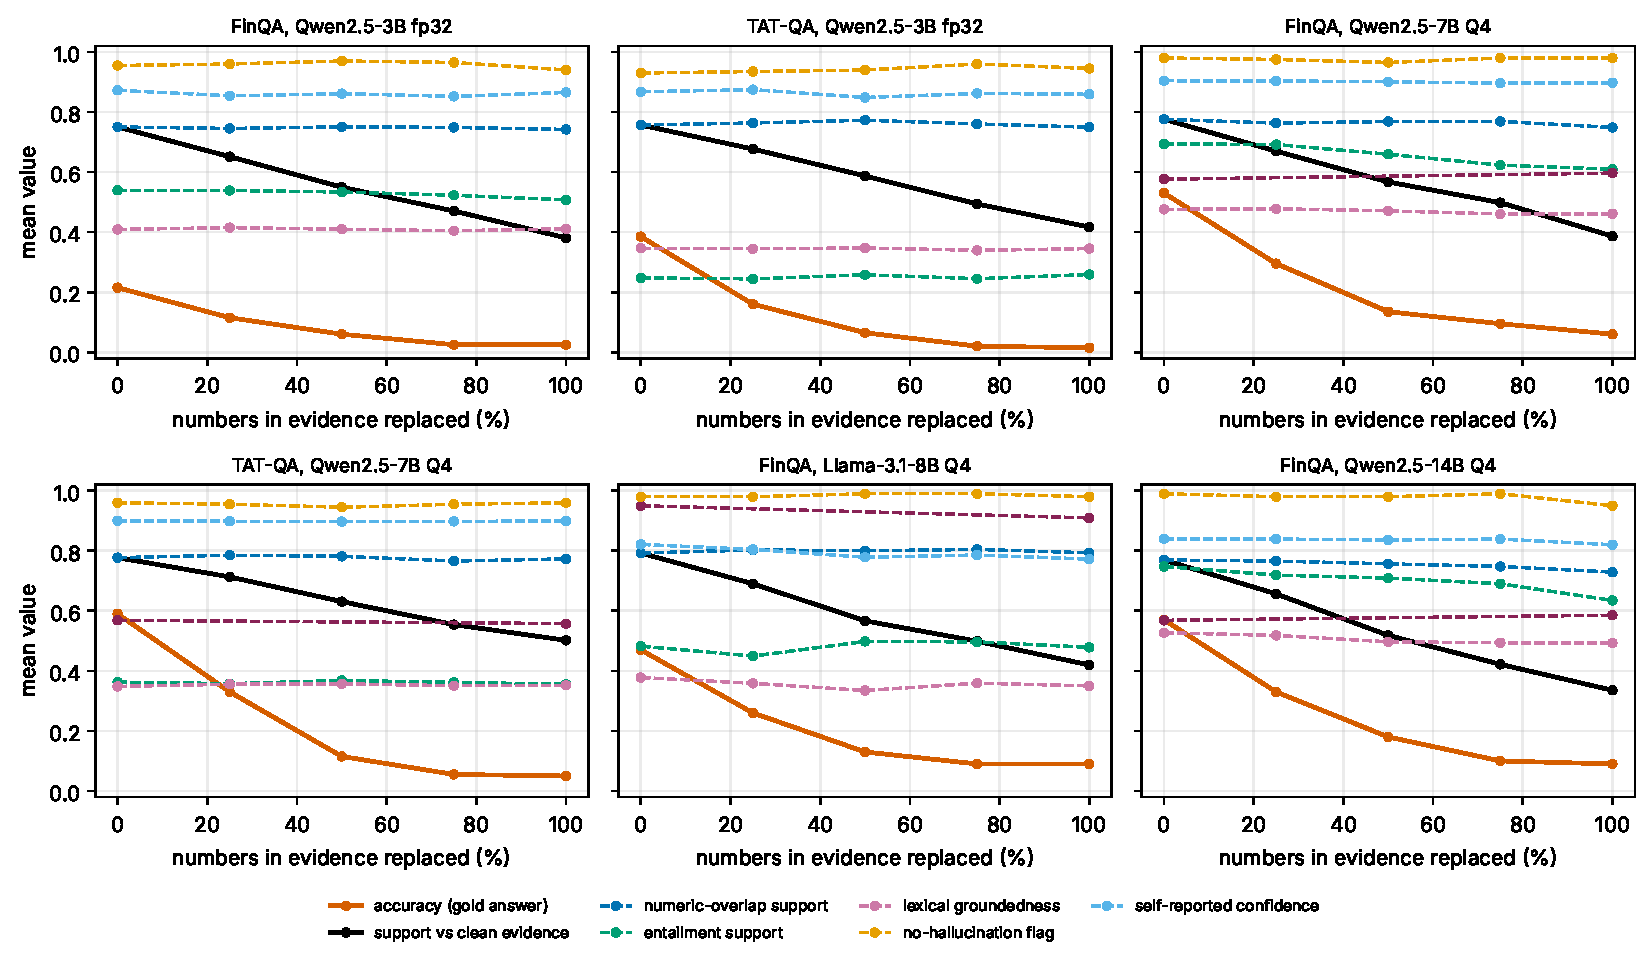
\includegraphics[width=\textwidth]{figures/corruption.pdf}
\caption{Mean value of each measure against the share of numbers in the retrieved evidence that were replaced by wrong ones (dev and test runs averaged within a dataset and model; 100 items per run). Solid lines need the gold answer or the clean evidence; dashed lines use only the response and the evidence shown to the model.}
\label{fig:corruption}
\end{figure}

Table~\ref{tab:paired} gives the paired change per item from $0\%$ to $100\%$ corruption.
Accuracy falls by 0.19 to 0.45 depending on run, and support against the clean evidence by 0.33 to 0.41.
The gold-free measures move by at most a few points.
For the 7B model, numeric-overlap and entailment support decline slightly but reliably (about $-0.03$ and $-0.09$), an order of magnitude less than accuracy.

\begin{table}[t]
\centering\small
\resizebox{\textwidth}{!}{\begin{tabular}{@{}l r ccccc@{}}
\toprule
Run & $n$ & accuracy$^\dagger$ & numeric-overlap support & entailment support & hallucination flag & support vs clean$^\ddagger$ \\
\midrule
FinQA / Qwen2.5-3B fp32 dev & 100 & -0.19 \small[-0.27, -0.12] & +0.00 \small[-0.02, +0.03] & +0.02 \small[-0.04, +0.07] & +0.01 \small[-0.04, +0.06] & -0.36 \small[-0.40, -0.33] \\
FinQA / Qwen2.5-3B fp32 test & 100 & -0.19 \small[-0.27, -0.11] & -0.02 \small[-0.06, +0.02] & -0.07 \small[-0.14, -0.00] & +0.02 \small[-0.03, +0.07] & -0.38 \small[-0.42, -0.33] \\
TAT-QA / Qwen2.5-3B fp32 dev & 100 & -0.37 \small[-0.46, -0.28] & +0.00 \small[-0.03, +0.03] & +0.04 \small[-0.02, +0.10] & -0.02 \small[-0.07, +0.03] & -0.35 \small[-0.39, -0.31] \\
TAT-QA / Qwen2.5-3B fp32 test & 100 & -0.37 \small[-0.46, -0.28] & -0.02 \small[-0.04, +0.01] & -0.02 \small[-0.08, +0.03] & -0.01 \small[-0.05, +0.02] & -0.33 \small[-0.36, -0.30] \\
FinQA / Qwen2.5-7B Q4 test & 100 & -0.45 \small[-0.55, -0.35] & -0.03 \small[-0.06, -0.01] & -0.09 \small[-0.16, -0.02] & +0.01 \small[-0.02, +0.05] & -0.41 \small[-0.44, -0.37] \\
TAT-QA / Qwen2.5-7B Q4 test & 100 & -0.58 \small[-0.68, -0.47] & -0.02 \small[-0.05, -0.00] & -0.03 \small[-0.09, +0.03] & +0.02 \small[-0.02, +0.06] & -0.29 \small[-0.33, -0.25] \\
FinQA / Llama-3.1-8B Q4 test & 100 & -0.38 \small[-0.48, -0.28] & +0.00 \small[-0.03, +0.03] & +0.00 \small[-0.07, +0.07] & +0.00 \small[-0.03, +0.03] & -0.37 \small[-0.41, -0.34] \\
\bottomrule
\end{tabular}}
\caption{Change from $0\%$ to $100\%$ corruption, paired within item, with 95\% bootstrap intervals over items. $^\dagger$ needs the gold answer. $^\ddagger$ needs the clean evidence.}
\label{tab:paired}
\end{table}

The question is whether a measure can \emph{tell} the two situations apart, not only whether its average moves.
Table~\ref{tab:corrupt-auroc} reports the AUROC for separating a response generated from fully corrupted evidence from one generated from the clean evidence of the same item.
Every gold-free measure is close to chance: pooled over runs, numeric-overlap support gives \aucFinoverlap{} \aucFinoverlapci{} on FinQA and \aucTatoverlap{} \aucTatoverlapci{} on TAT-QA, entailment support \aucFinnli{} and \aucTatnli{}, and the hallucination flag \aucFinnohalluc{} and \aucTatnohalluc{}.
Individual runs reach at most 0.58.
Accuracy, which needs the gold answer, reaches \aucFincorrect{} and \aucTatcorrect{} (it is limited because many clean responses are already wrong), and support against the clean evidence reaches \aucFinvsclean{} and \aucTatvsclean{}.
The information that distinguishes the two cases is in the pair (response, clean evidence), which a deployed system does not have.

\begin{figure}[t]
\centering
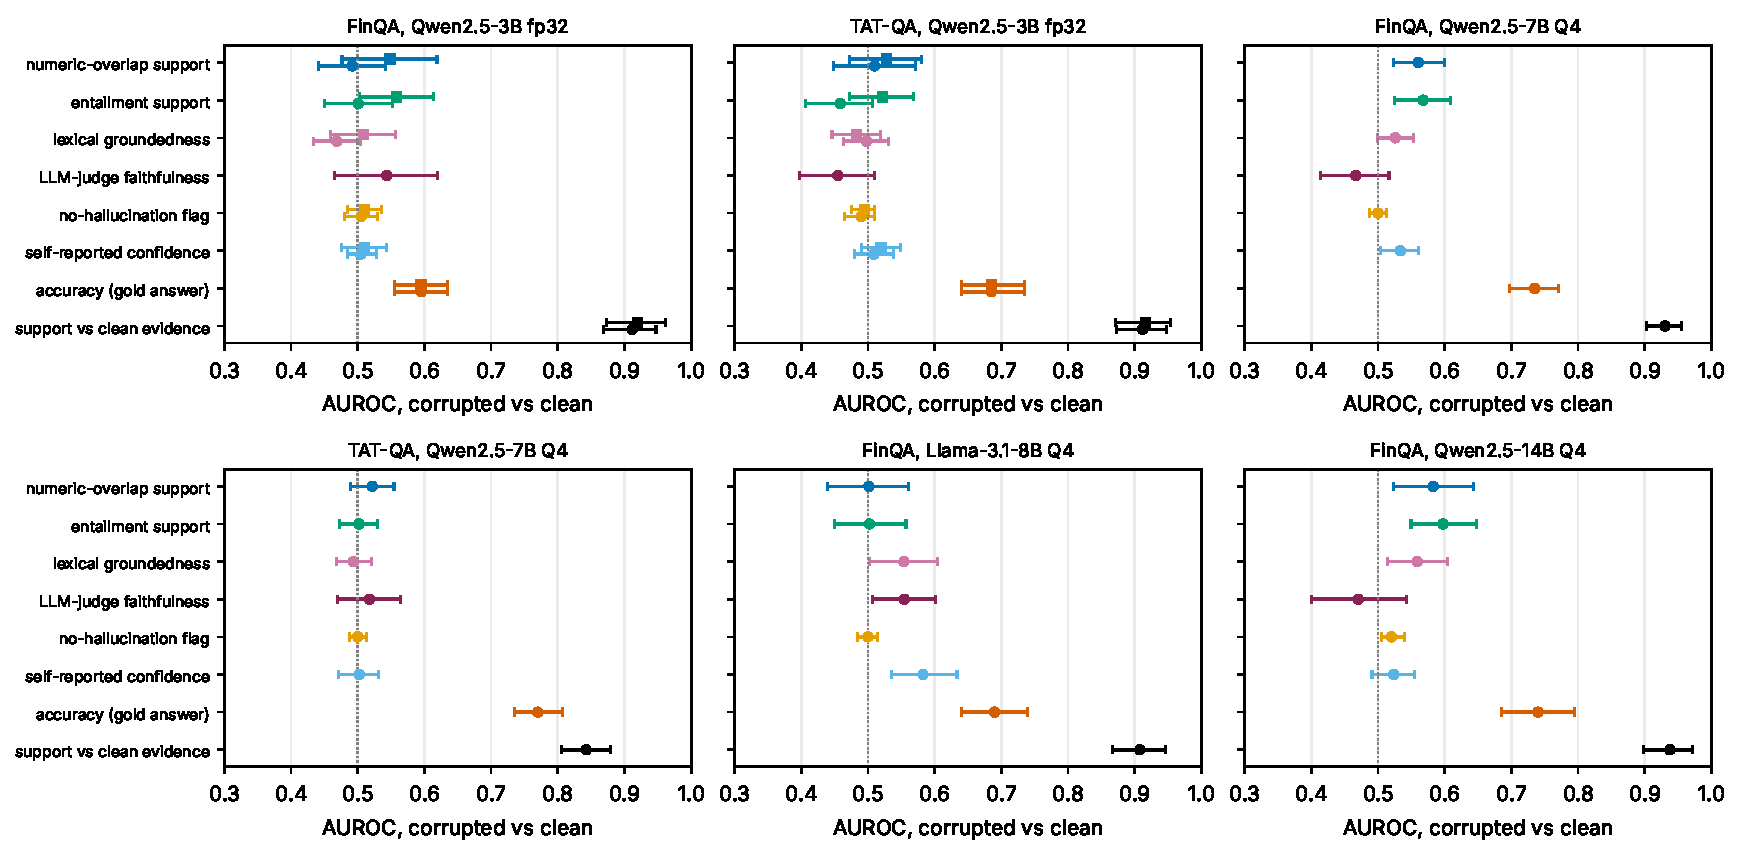
\includegraphics[width=\textwidth]{figures/auroc.pdf}
\caption{AUROC for telling a response produced from $100\%$-corrupted evidence from one produced from clean evidence (95\% bootstrap intervals over items; one marker per run). The dotted line is chance.}
\label{fig:auroc}
\end{figure}

\begin{table}[t]
\centering\small
\resizebox{\textwidth}{!}{\begin{tabular}{@{}l r ccccccc@{}}
\toprule
Run & $n$ & numeric-overlap support & entailment support & lexical groundedness & no-hallucination flag & self-reported confidence & accuracy$^\dagger$ & support vs clean$^\ddagger$ \\
\midrule
FinQA / Qwen2.5-3B fp32 dev & 100 & 0.49 \small[0.44, 0.54] & 0.50 \small[0.45, 0.55] & 0.47 \small[0.43, 0.50] & 0.51 \small[0.48, 0.53] & 0.50 \small[0.48, 0.52] & 0.59 \small[0.56, 0.64] & 0.91 \small[0.87, 0.95] \\
FinQA / Qwen2.5-3B fp32 test & 100 & 0.55 \small[0.48, 0.63] & 0.56 \small[0.51, 0.62] & 0.51 \small[0.46, 0.55] & 0.51 \small[0.49, 0.54] & 0.51 \small[0.48, 0.54] & 0.59 \small[0.55, 0.63] & 0.92 \small[0.87, 0.96] \\
\midrule
FinQA pooled & 200 & 0.52 \small[0.48, 0.57] & 0.53 \small[0.50, 0.57] & 0.49 \small[0.46, 0.51] & 0.51 \small[0.49, 0.53] & 0.51 \small[0.49, 0.53] & 0.59 \small[0.57, 0.62] & 0.92 \small[0.89, 0.94] \\
\bottomrule
\end{tabular}}
\caption{AUROC (95\% interval) for separating $100\%$-corrupted from clean evidence. $^\dagger$ needs the gold answer. $^\ddagger$ needs the clean evidence. Pooled rows combine the runs above them.}
\label{tab:corrupt-auroc}
\end{table}

The composite behaves accordingly.
Its correlation with the corruption level over the five levels is between $-0.90$ and $-0.97$ in every run, with intervals that exclude zero, and it comes entirely from the accuracy term and from the calibration term, which is a function of accuracy.
Replacing numeric-overlap support by support against the clean evidence in the composite changes little, because the composite is already dominated by accuracy.
So the composite does fall with corrupted evidence, but only through the terms that need the gold answer.

\subsection{Detecting wrong answers on clean evidence}

On clean evidence the gold-free measures should be useful if they carry information about errors.
Table~\ref{tab:error} shows they carry little.
Pooled over runs, AUROC for separating correct from incorrect answers is \errFinoverlap{} for numeric-overlap support, \errFinnli{} for entailment support, \errFinlexical{} for lexical groundedness, \errFinnohalluc{} for the hallucination flag and \errFinconf{} for verbalized confidence on FinQA (TAT-QA: \errTatoverlap, \errTatnli, \errTatlexical, \errTatnohalluc, \errTatconf).
Some individual runs deviate from 0.5 in both directions; for the 7B model numeric-overlap support is \emph{below} 0.5 on FinQA, because correct answers contain a computed result that is, by construction, not in the evidence, while a wrong answer that merely copies a figure scores as fully supported.
Verbalized confidence is nearly constant (most responses say 0.9), so its AUROC is uninformative regardless of model.
The lexical baseline performs no better than the entailment or overlap scores, so the weakness is not particular to the numeric-overlap design.

\begin{table}[t]
\centering\small
\resizebox{\textwidth}{!}{\begin{tabular}{@{}l r r ccccc@{}}
\toprule
Run & $n$ & Acc. & numeric-overlap support & entailment support & lexical groundedness & no-hallucination flag & self-reported confidence \\
\midrule
FinQA / Qwen2.5-3B fp32 dev & 100 & 0.22 & 0.60 \small[0.46, 0.73] & 0.49 \small[0.36, 0.62] & 0.52 \small[0.41, 0.65] & 0.53 \small[0.51, 0.56] & 0.53 \small[0.49, 0.59] \\
FinQA / Qwen2.5-3B fp32 test & 97 & 0.22 & 0.47 \small[0.32, 0.62] & 0.57 \small[0.43, 0.71] & 0.62 \small[0.48, 0.74] & 0.50 \small[0.44, 0.54] & 0.50 \small[0.47, 0.54] \\
FinQA / Qwen2.5-3B fp32 dev & 149 & 0.26 & 0.64 \small[0.55, 0.73] & 0.53 \small[0.43, 0.63] & 0.48 \small[0.38, 0.57] & 0.53 \small[0.51, 0.55] & 0.53 \small[0.49, 0.57] \\
FinQA / Qwen2.5-3B fp32 test & 145 & 0.21 & 0.52 \small[0.41, 0.64] & 0.55 \small[0.44, 0.67] & 0.57 \small[0.44, 0.69] & 0.51 \small[0.47, 0.54] & 0.53 \small[0.49, 0.58] \\
FinQA / Qwen2.5-1.5B fp32 dev & 100 & 0.40 & 0.44 \small[0.33, 0.54] & 0.51 \small[0.41, 0.61] & 0.46 \small[0.35, 0.59] & 0.52 \small[0.47, 0.56] & 0.53 \small[0.44, 0.61] \\
FinQA / Qwen2.5-1.5B fp32 test & 97 & 0.34 & 0.48 \small[0.36, 0.60] & 0.50 \small[0.39, 0.61] & 0.48 \small[0.35, 0.60] & 0.54 \small[0.51, 0.57] & 0.55 \small[0.45, 0.63] \\
FinQA / SmolLM2-1.7B fp32 dev & 100 & 0.16 & 0.32 \small[0.20, 0.47] & 0.42 \small[0.26, 0.61] & 0.36 \small[0.24, 0.52] & 0.47 \small[0.38, 0.54] & 0.50 \small[0.50, 0.50] \\
\midrule
FinQA pooled & 788 & 0.25 & 0.50 \small[0.46, 0.55] & 0.51 \small[0.47, 0.55] & 0.51 \small[0.47, 0.55] & 0.52 \small[0.50, 0.53] & 0.54 \small[0.52, 0.57] \\
\bottomrule
\end{tabular}}
\caption{AUROC for separating correct from incorrect answers under clean evidence (numeric questions only; 95\% bootstrap intervals over items).}
\label{tab:error}
\end{table}

\subsection{Real retrieval misses}

Corruption is synthetic.
A natural failure of the same kind occurs when the retriever does not surface the numbers the answer needs.
Table~\ref{tab:retrieval} compares items by whether the retrieved evidence contains every number of the gold evidence.
The miss rate is $\approx$\missFin\% on FinQA and varies by dataset definition on TAT-QA.
Accuracy is much lower on misses than on hits.
Whether a gold-free measure notices is inconsistent: pooled over FinQA runs numeric-overlap support gives AUROC \retFinoverlap{}, entailment \retFinnli{}, lexical groundedness \retFinlexical{}; for the 3B model on TAT-QA numeric-overlap support reaches 0.69, because with the needed figures absent the model invents or substitutes numbers that are then not in the evidence.
That is a different failure from corrupted evidence: \emph{missing} evidence can leave a trace in the response, whereas \emph{wrong} evidence leaves none.
Even where overlap support helps, accuracy itself separates hits from misses at least as well (FinQA pooled \retFincorrect).

\begin{table}[t]
\centering\small
\resizebox{\textwidth}{!}{\begin{tabular}{@{}l r r r cccccc@{}}
\toprule
Run & $n$ & Miss & Acc. hit / miss & numeric-overlap support & entailment support & lexical groundedness & no-hallucination flag & self-reported confidence & accuracy$^\dagger$ \\
\midrule
FinQA / Qwen2.5-3B fp32 dev & 150 & 0.13 & 0.29 / 0.00 & 0.53 \small[0.38, 0.68] & 0.60 \small[0.48, 0.70] & 0.48 \small[0.34, 0.61] & 0.53 \small[0.47, 0.60] & 0.61 \small[0.52, 0.72] & 0.65 \small[0.61, 0.69] \\
FinQA / Qwen2.5-3B fp32 test & 150 & 0.20 & 0.23 / 0.07 & 0.59 \small[0.47, 0.71] & 0.49 \small[0.38, 0.60] & 0.43 \small[0.29, 0.56] & 0.51 \small[0.47, 0.56] & 0.47 \small[0.38, 0.54] & 0.58 \small[0.52, 0.63] \\
FinQA / Qwen2.5-1.5B fp32 dev & 100 & 0.12 & 0.44 / 0.08 & 0.51 \small[0.32, 0.69] & 0.47 \small[0.30, 0.66] & 0.43 \small[0.23, 0.61] & 0.51 \small[0.45, 0.61] & 0.36 \small[0.22, 0.51] & 0.68 \small[0.56, 0.76] \\
FinQA / Qwen2.5-1.5B fp32 test & 100 & 0.17 & 0.39 / 0.06 & 0.57 \small[0.41, 0.73] & 0.58 \small[0.43, 0.73] & 0.48 \small[0.35, 0.64] & 0.54 \small[0.47, 0.63] & 0.44 \small[0.31, 0.56] & 0.66 \small[0.58, 0.73] \\
FinQA / SmolLM2-1.7B fp32 dev & 100 & 0.12 & 0.18 / 0.00 & 0.47 \small[0.30, 0.65] & 0.56 \small[0.43, 0.70] & 0.44 \small[0.26, 0.60] & 0.45 \small[0.42, 0.48] & 0.50 \small[0.50, 0.50] & 0.59 \small[0.56, 0.63] \\
\midrule
FinQA pooled & 600 & 0.15 & 0.30 / 0.04 & 0.54 \small[0.47, 0.61] & 0.53 \small[0.47, 0.59] & 0.45 \small[0.38, 0.52] & 0.51 \small[0.49, 0.54] & 0.48 \small[0.43, 0.52] & 0.63 \small[0.59, 0.65] \\
\bottomrule
\end{tabular}}
\caption{Items split by whether the retrieved evidence contains every number of the gold evidence (FinQA: annotated gold facts; TAT-QA: operands of the annotated derivation). AUROC: can the measure tell complete from incomplete retrieved evidence? $^\dagger$ needs the gold answer.}
\label{tab:retrieval}
\end{table}
